\title{Impera}
\author{
        Paul F Baumeister}
\date{\today}



\documentclass[12pt]{article}

\usepackage{todonotes}
\usepackage{amsmath}
\usepackage{amssymb}
\usepackage{bbm}
\usepackage{booktabs}
% \usepackage{graphics}
\usepackage{tikz} %%% nice plots if the function is known
% \usepackage{here}
\usepackage{units} %%% for nicefrac
\usepackage{todonotes}


\newcommand{\ttt}[1]{\texttt{#1}}
\newcommand{\um}[1]{_{\mathrm{#1}}}
\newcommand{\derive}[2]{\frac{\partial #1}{\partial #2}}


\begin{document}
\maketitle

\begin{abstract}
Impera tries to find a parametrization
that describes the dynamics of populations
and mimiques the rise and fall of empires
as observed in world history of the past four millennia.
\end{abstract}

\section{Introduction}
How simple can a model of world
population be which is still capable
of reproducing some of the phenomena that we
can observe studying the history on an abstract
scale. 
The abstraction refers to similar 
concepts of how political power can be
used.

\paragraph{Outline}
The remainder of this article is organized as follows.
Section~\ref{sec:previous_work} gives account of previous work.
Our new and exciting results are described in Section~\ref{sec:results}.
Finally, Section~\ref{sec:conclusions} gives the conclusions.


\section{Previous work} \label{sec:previous_work}
If there were previous work on this I had found in the
accessible literature, I would maybe take that.

\section{General thoughts} \label{sec:general_thoughts}
Hypothesis: A population is efficient as long as they dont live too good.
Once they gain economical power, they get richer, live better, become
greedy and then it starts to drop like all empires disappeared and 
will continue to cease after some time.
Most populations keep a slave race to do the dirty work.
As slave race, the efficiency to gain power is suppressed,
but they become more efficient by mass since the master race
does not procreate, dies in wars or becomes collectively insane (degenerates).

This means, we only have two numbers per species living in one region:
population number and power. The higher the power, the faster grows
a populations wealth\&power\&degeneracy.
A war kills population and reduces wealth\&power\&degeneracy.
the more a populations resources are limited, the faster it tries to
expand. This is realized via a diffusion process.

all populations of a species are connected across the whole planet.
the power of a race is omni-present, i.e. if one race attacs a suppressing
leadership minority, the mainland will strike back.
How can we mimique over-critical states? This is a question of hysteresis.

The more people use a resource, the slower they can grow.
Obviously, this happened to the roman empire.
A periodic function that grows exponentially and then drops heavily or
a sawtooth function in time. 
If all population of a species gets killed, a new species is born (where?), so the
total number of species on earth stays constant.
Between regions, populations of the same species have a strong diffusion
coefficient for their wealth (supply the oversee provinces with support).
races tend to move towards free resources and away from other strong species.
A master species tries to have a slave species in the same region
and then, when the slaves have become too mighty, they cannot keep
them down any more.

As globalization proceeds, the masters may be a tiny minority
of the population of the imperialistic country that live in and rule
a colony
when a species is strong, the diffusion into other countries must be
as large as the others fight back.
The technology level defines, which of the resources are economically
important now

the larger the ratio of powers, the more power can a race extract from
the suppressed one

the master race always fears the slace race and the slave race hates the masters
up to the point where the masters become weak because they have
degenerated in their greed.

the masters power is by definition higher than that of the slaves,
so the slaves will have to give their products to the masters (at no returned values)
This makes the masters need the slaves, so the masters can attract slaves (i.e. buy them)

the higher the power difference is, the more of the generated power is transferred to
the master, therefore, a colony will stay weak for very long before becoming independent.

one could think of the master power to be radiated from the mainland

Although all colonies have become independent, the economic trade relations are still in place
to let the money/power flow, so basically nothing has changed.

diffusion into other countries is high, if the resources are low.
migration into other regions always means war.
define the resistance against diffusion: power $\times$ population of the target region

what are the effects that need to occur to replay world history?
 - slavory: a powerful species keeps a worker species like prisoners 
 - guest workers: a powerful species keeps a worker species
 - repelling: a minority is repelled more the stronger the majority is
 - rioting: a large population throws over a minority rulership
 - invasion: a stronger species can always invade another region
 - aggression: the more populated a region, the more aggressive
 - degeneracy: a species that is too powerful will not procreate longer
 - power is extrinsic or at least shared among some distance
 - expansion: if a population density is too high, they diffuse
 - you can invade/enter a country as far more or far less powerful
 - if you are more powerful, they'll fight you
 - if you are less powerful, they'll welcome you
 - an isolated population will live in peace and grow exponentially
 - until the resources are reached, then they will not grow further
 - and will start to diffuse stronger
 - raids powerful fighters (e.g.~Goths) live on the wealth of others
 - diaspora
 - the slaves also increase their power while serving
 - express it as a pair relation between two species
 - resources define the pressure
 - once we move into the society of services, regions do not matter
 that much any more since power radiates further

 - two species: $M$,$m$
 - $M$ is the Majority, $m$ is the minority
 - if $p_M > p_m$ (majority rule): 
      most of the power generated by $m$ is transferred to $M$
      $m$ tries to flee, if possible (enough power to enter another region)
 - else (minority rule):
      most of the power generated by $M$ is transferred to $m$
      $M$ tries to flee
 - successful diffusion increases power (technology bonus)
 - living on an isolated island just doesnt bring you power

 - Fertility $F(P) = F_{max} \cdot \left( 1 - \left(\frac{P}{P_{max}} \right)^2 \right)$ with $F_{max}$ around 5 percent per year,
    times the gain in power, as first step, we can set $f_{max}$ to infinity

\begin{figure} [ht]
  \centering
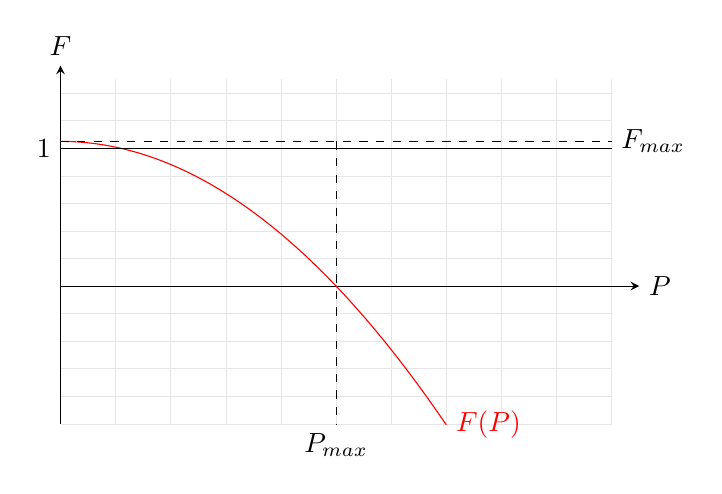
\begin{tikzpicture}[scale=3.5, yscale=0.5, domain=0:2, >=stealth]
  \draw[step=.2, color=black!10, very thin] (0,-1) grid (2,1.5);
  \draw[->] (0,0) -- (2.1,0) node[right] {$P$};
  \draw[->] (0,-1) -- (0,1.6) node[above] {$F$};
  \draw[color=red] plot[smooth,samples=99,domain=0:1.4] (\x,{1.05*(1-\x*\x)}) node[right] {$F(P)$};
  \draw[-, color=black] (2,1) -- (0,1) node[left] {$1$};
  \draw[-, color=black, dashed] (0,1.05) -- (2,1.05) node[right] {$F_{max}$};
  \draw[-, color=black, dashed] (1,1.05) -- (1,-1) node[below] {$P_{max}$};
\end{tikzpicture}
  \label{fig:harvest_function}
  \caption{Fertility $F$ as a function power $P$. The formula is $ F(P) = F_{max} \left( 1 - \left(\frac{P}{P_{max}} \right)^2 \right) $
  with $F_{max}$=1.05, so a $5\,\%$ growth. For powers that exceed $P_{max}$, the growth is even negative, i.e.~more people die than children are born.
  The model is the antagonist of the growing power. Since strength density can only grow, the total strength of a population will decrease once
  the population becomes too powerful.
  } 
\end{figure}  
    
    
 - a population lets a weaker population enter a country, if 
    the weaker ones bring a benefit to the existing population
    the transfer rate is ~ $p_m$ - $p_M$
   the diffusion barrier is larger, more the power are equal:
 - diffusion barrier ~ $(\log(p_m/p_M))^2$ is scale invariant

 - there is a maximum population $P$ that a region can feed 
defined by the resources $R$, i.e. the local gain of power
is defined as $G = \frac{2 \cdot R \cdot P}{R + P}$
here, the factor $2$ is chosen arbitraryly. This value affects that
an isolated region would be able to produce nutrition for a population
of magnitude $P$=$R$.

 - the distribution of the Gain to the populations happens according
   to their powers, i.e.
   population $j$ gets $w_j = \frac{ p_j \cdot f_j }{ \sum_i p_i \cdot f_i }$

- the pressure that generates diffusion comes from the how much less
  gain is there than needed to maintain fertility

- the question is always: how can a population increase his strength $p \cdot f$

- P is radiated across the grid, i.e. there is a diffusion that is
  stronger ther faster communication is. Communication speed could
  depend on the total power --> non-linear, capitalistic effect

- the amount of fighting $F \propto \log^2 \left( \frac{p_m \cdot f_m}{p_M \cdot f_M} \right)$
  because you would not start a fight, if your power is much lower
  than and you don't need to fight if you are much more powerful, 
cause then you can work with threat
 - the fighting reduces the 
        +strength $p_M \cdot f_M$ by $F$ and $p_m \cdot f_m$ by $F$ and the 
		+population $p_M$ by $\frac{ p_M^2 }{ p_m }$ and $p_m$ by $\frac{ p_m^2 }{ p_M }$ because
  the more powerful, the more efficient are the weapons.
  So far, $F$ is unitless. However, we would like to find a formula
  such that almost only power is reduced at the powerful species and almost only
  population is reduced at the numerous species. Assume that the fighting $F$
  is maximum ($F=1$) since the strengths are equal, then, there is only one
  parameter left that determines the ratio of powers and populations,
  which we call $k$.


- if two species are friendly, the stronger one will take a large part
  of the gains from the weaker one and the hostility grows.
- if two species are hostile, there is a fight and the hostility grows
- if two species are both hostile to a third one, they put down their
mutual hostility to save forces
- all new species start as friends (positive baseline attitude)

- power lets the diffusion barriers due to distance or terrain appear
  small, really powerfull species will fly anywhere anyway
- the map contains natural diffusion barriers.
- coastlines are connected among each other - barrier = seaway distance

- if a species got extinct, there is an exile and the last remaining
  human of that species is transferred to the least populated area of
  the planet and assigned with a power slightly larger than that of
  any potential species present there. All hostility is set to
  max. friendly
  alternatively, once there is a free slot for a species, one could
  measure
  how much the regions are paying to their crown and try to see if
  there
  is a big discrepancy between colonies and mainland. if so, we can
  separate. this involves transferring most of the populations in a
  selected set of regions where the saldo was negative

- being in contact leaks power if the attitude is friendly
- forgiving and forgetting: attitude goes back to friendly with time (roughly over $10$ generations)

\begin{itemize}
 \item compute the harvest from the total population of the region
 \item compute the part of the harvest that goes to each of the species
 \item compute the unfairness of this partitioning for the change of hostility
 \item compute the change in population and in power
 \item compute the local diffusion of power depending on hostility
 \item compute the percentage of diffusors depending on local conditions
 \item compute the local living condition
 \item compute the diffusion gradient and barrier for each of the neighboring regions
 \item propagate diffusors
 \item radiate the power
 \item compute the need to fight
 \item compute the casulties and lost strength ($P \cdot M$)
 \item compute population growth and power increase
\end{itemize}


- different time scales, i.e.
- the intersting phase starts around 9483 BC running $2^{22}$ days to come back into the present
- we can also start earlier, e.g. 20966 BC running $2^{23}$ days to come back into the present
- the time step should decrease on a log scale (because that is how
- humans perceive it), i.e. it the time scale 


\begin{table} [ht]
  \centering
\begin{tabular}{ c c c c }
\hline  
%Start-year &
  End-year & Time Step in Days & Time step & Era \\
\hline  
   -43919  & $2^{11} = 2048$ &  6 years & Middle Stone Age \\ 
   -20952  & $2^{10} = 1024$ &  3 years & Late Stone Age \\ % Upper Paleolithic
    -9469  & $2^9 = 512$ &  1$\nicefrac{1}{2}$ years & Late Stone Age \\ % Upper Paleolithic and Proto-Neolithikum
    -3727  & $2^8 = 256$ &  $\nicefrac{2}{3}$ year & New Stone Age and Copper Age \\ %% Neolithic is -10200 to -4500
     -856  & $2^7 = 128$ &  4 months & Bronce Age \\ 
      578  & $2^6 = 64$ &  2 months & Iron Age \\ % and beginning Early Middle Age
     1296  & $2^5 = 32$ &  1 month & Middle Age \\ % Early Middle Age and High Middle Age
     1655  & $2^4 = 16$ &  2 weeks & Renaissance \\ % European Renaissance (about 1420–1630), Reformation and Counter-reformation
     1834  & $2^3 = 8$ &  1 week & Enlightenment \\ 
     1924  & $2^2 = 4$ &  4 days & Imperialism \\ % and industrialization
     1969  & $2^1 = 2$ &  2 days & WWII \\ 
     2014  & $2^0 = 1$ &  1 day & Cold war and Present \\ 
\hline 
\end{tabular} 
  \label{tab:time_steps_for_ages}
  \caption{Ages are treated with different time steps following an exponential function.
  The more it is in the past, the longer is the step in time 
  so that all ages take $2^{13} (\approx$ eight thousand) time steps.} 
\end{table}
\todo[inline]{shift all years by -14, end of Imperalism should be 1910 and then there is the era of WWI and WWII until 1955 or shift all by +21 (then 2035, 1990, 1945).} 



we need staedy states:
The distribution of harvest is such that the slaves don't die of hunger but also don't gain power
if there is not enough food, the more powerful will take as much as he
needs and let the slaves die, if necessary.

The conditions for living are determined by the ratio of work and gain

\begin{figure} [ht]
  \centering
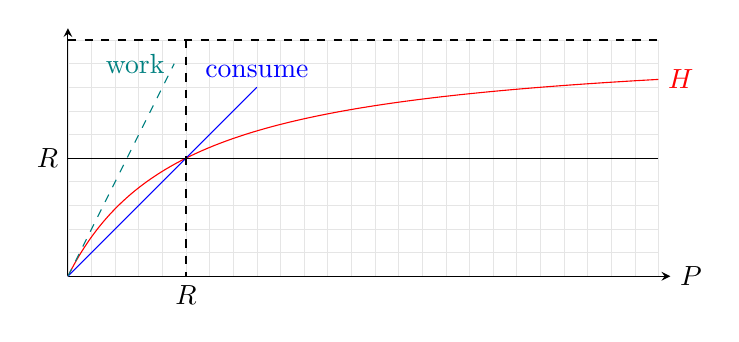
\begin{tikzpicture}[scale=1.5, domain=0:5, >=stealth]
%   \draw[step=.2, color=lightgray, very thin] (0,0) grid (5,2);
  \draw[step=.2, color=black!10, very thin] (0,0) grid (5,2);
  \draw[->] (0,0) -- (5.1,0) node[right] {$P$};
  \draw[->] (0,0) -- (0,2.1);
  \draw[color=red] plot[smooth,samples=99] (\x,{2.0*\x/(1.0+\x)}) node[right] {$H$};
  \draw[-, color=blue] (0,0) -- (1.6,1.6) node[above] {consume};
  \draw[-, color=teal, dashed] (0,0) -- (.9,1.8) node[left] {work};
  \draw[-, color=black] (5,1) -- (0,1) node[left] {$R$};
  \draw[-, color=black, dashed] (0,2) -- (5,2);
  \draw[-, color=black, dashed] (1,2) -- (1,0) node[below] {$R$};
\end{tikzpicture}
  \label{fig:harvest_function}
  \caption{The local harvest $H$ is a function of the local total population $P$ 
  and the local resources $R$. 
  The population $P$ consumes $P$ to survive and provides a work force 
  large enough to harvest twice as much as for $P \ll R$. 
  The crossover happens exactly at $P=R$ since the harvest function chosen here is
  $H(P) = \frac{2RP}{R+P}$.
  } %%% the work force F could also be scaled freely,
\end{figure}  


$P$ total local population $P = \sum_i p_i$ \\
$s_i$ strength $s_i = p_i \cdot f_i$ \\
$S$ total strength $S = \sum_i s_i$ \\
$f_i$ force \\

my share of the harvest $H$ with the weight $w_i$.
I consume $p_i$ of that, i.e. my contribution $C_i$ to the crown $i$ is
  $$ C_i = s_i/S \cdot H-p_i = \frac{p_i \cdot f_i}{\sum_j p_j \cdot f_j} \cdot  \frac{2 \cdot R \cdot \sum_j p_j}{R+\sum_j p_j} - p_i $$
with $P = \sum_j p_j$.
How can I increase $C$?
We construct the partial derivatives w.r.t.~$p_j$ -- we assume $f_j$ so vary only adiabatically
if the resources are below limits, more workers are good to increase the gain
\begin{align}
\derive{H}{P} &= \frac{2R}{R+P} - \frac{2R \cdot P}{(R+P)^2} = \frac{2 R^2}{(R+P)^2} \\
\derive{P}{p_i} &= 1 \quad \text{and} \quad \derive{S}{p_i} = f_i \quad \text{and} \quad w_i = \frac{s_i}{S} \\
\derive{w_i}{p_j} &= \frac{\delta_{ij} f_i^2 - f_j \cdot s_i}{S^2}
\intertext{Matrix of interests (comment: the last $f_i$ can be exchanged to $f_j$)}
\derive{C_i}{p_j} &= \frac{2 \cdot R^2}{(R+P)^2} \cdot w_i -  \frac{w_i \cdot f_j}{S} + \delta_{ij} \cdot ( \frac{f_i}{S} - 1 )
\end{align}

the interest diagonals control the balance between diffusion and
acceptance, 
the off-diagonal elements control warfare and trade-relations
the diffusion barriers can be weighted according to rulership weights $w_i$ (is
this needed? most of the terms carry a $w_i$ already)

for two species: with $s_M = p_M \cdot f_M$ and $s_m = p_m \cdot f_m$
\begin{align}
\derive{C_m}{p_m} &= 2 \cdot R^2/(R+p_M+p_m)^2 \cdot s_m/S - s_m/S \cdot f_m/S + f_m/S - 1 \\
\derive{C_m}{p_M} &= 2 \cdot R^2/(R+p_M+p_m)^2 \cdot s_m/S - s_m/S \cdot f_M/S \\
\derive{C_M}{p_m} &= 2 \cdot R^2/(R+p_M+p_m)^2 \cdot s_M/S - s_M/S \cdot f_m/S \\
\derive{C_M}{p_M} &= 2 \cdot R^2/(R+p_M+p_m)^2 \cdot s_M/S - s_M/S \cdot f_M/S + f_M/S - 1 \\
\end{align}


%\begin{figure} [ht]
%  \centering
%\begin{tikzpicture}[scale=10]
%  \draw[step=.02, gray, very thin] 
%  (-0.1,-0.1) grid (1.1,0.15);
%
%  \draw[color=red, domain=0.:1., scale=5] 
%    plot[id=naca] 
%      (\x,{0.12/0.2*(0.2969*sqrt(\x )-0.126*\x -0.3516*\x^2 +0.2843*\x^3 -0.1015*\x^4 )});
%  
%  \draw[color=blue, domain=0.:.05, yshift=1] 
%    plot[id=naca] 
%      (\x,{0.12/0.2*(0.2969*sqrt(\x )-0.126*\x -0.3516*\x^2 +0.2843*\x^3 -0.1015*\x^4 )});
%
%  \tikz \draw[thick,rounded corners=8pt] 
%      (0,0) -- (0,2) -- (1,3.25) -- (2,2) -- (2,0) -- (0,2) -- (2,2) -- (0,0) -- (2,0);
%
%  \usetikzlibrary[trees]
%  \node {root}
%  [clockwise from=30,sibling angle=30]
%  child {node {$30$}}
%  child {node {$0$}}
%  child {node {$-30$}}
%  child {node {$-60$}};
%  
%\end{tikzpicture}
%  \label{fig:}
%  \caption{.}
%\end{figure}  


\begin{figure} [ht]
  \centering
  
  \begin{minipage}[l]{.59\textwidth}
  
    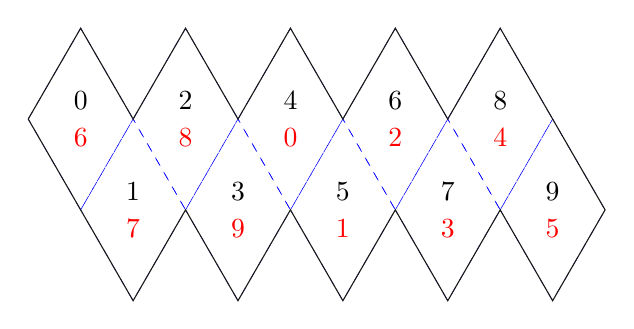
\begin{tikzpicture}[scale=0.666, yscale=.866, domain=0:11] %%% yscale enforces sqrt(3)/2 ratio for correct triangle height
      %%% plot northern rhombs
      \foreach \s in {0, 2, 4, 6, 8}{
        \draw[dashed, color=blue, very thin] (\s,1) -- (1+\s,3) -- (2+\s,1) -- (1+\s,-1) -- (\s,1);
        \node[above] at (1+\s,1) {\s};
      }
      %%% plot southern rhombs
      \foreach \s in {1, 3, 5, 7, 9}{
        \draw[dashed, color=blue, very thin] (\s,-1) -- (1+\s,1) -- (2+\s,-1) -- (1+\s,-3) -- (\s,-1);
        \node[above] at (1+\s,-1) {\s};
      }
      %%% alternative labels
      \foreach \s in {0, 2, 4}{ \node[below, color=red] at (5+\s, 1) {\s}; }
      \foreach \s in {6, 8}   { \node[below, color=red] at (\s-5, 1) {\s}; }
      \foreach \s in {1, 3, 5}{ \node[below, color=red] at (5+\s,-1) {\s}; }
      \foreach \s in {7, 9}   { \node[below, color=red] at (\s-5,-1) {\s}; }
      %%% plot solid line around all rhombs
      \draw[color=black!90, solid] (0,1) -- (1,3) -- (2,1) -- (3,3) -- (4,1) -- (5,3) -- (6,1) -- (7,3) -- (8,1) -- (9,3) -- (10,1) 
           -- (11,-1) -- (10,-3) -- (9,-1) -- (8,-3) -- (7,-1) -- (6,-3) -- (5,-1) -- (4,-3) -- (3,-1) -- (2,-3) -- (1,-1) -- (0,1);
    \end{tikzpicture}

  \end{minipage}
  \begin{minipage}[r]{.39\textwidth}
  
    \tiny
    \begin{tabular}{ll}
    \hline
      0 & Europe, N Africa, W Africa \\
      1 & E Africa, S Africa, SW Indian O \\
      2 & C Asia, Gulf, India, N Indian O \\
      3 & S Asia, C Australia, SE Indian O \\
      4 & E Asia, W Pacific O \\
      5 & New Zealand, Oceania, SW Pacific O \\
      6 & NE Pacific, N American W Coast \\
      7 & SE Pacific O \\
      8 & N America, C America, N Atlantic O \\
      9 & S America, SW Atlantic O \\
    \hline
    \end{tabular}
    \normalsize
    
  \end{minipage}
  \label{fig:world_map_on_icosahedral_grid}
  \caption{Unfolding of the icoahedron surface map. The canonical ordering of the ten rhombs is given with black labels. The red labels
  present the Europe-centered map with the Americas on the left hand side and Asia on the right. The table shows which continental
  parts can be found in which rhomb number. North, South, West, East, Central and Ocean are abbreviated.
  } %%% 
\end{figure}  




\begin{figure} [ht]
  \centering
  
  \begin{minipage}[l]{.49\textwidth}
  
    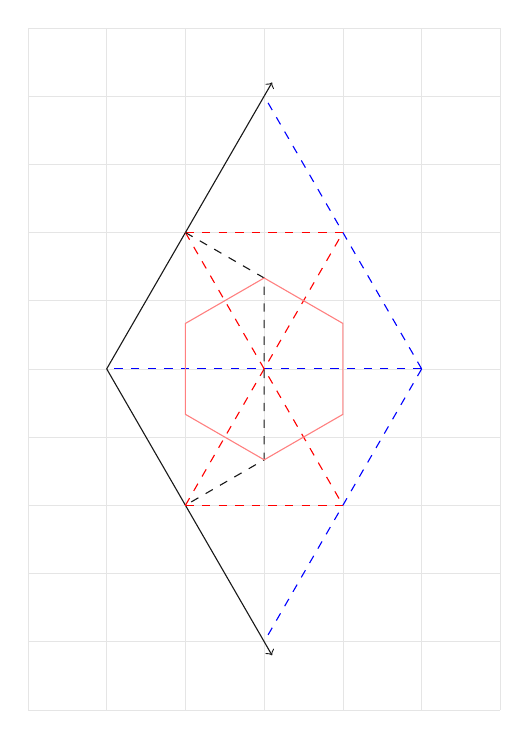
\begin{tikzpicture}[scale=1, yscale=.866, domain=0:4] %%% yscale enforces sqrt(3)/2 ratio for correct triangle height
      \draw[step=1.0, color=black!10, very thin] (-1,-5) grid (5,5);
      %%% plot northern rhombs
      
      \draw[<->, color=black!90, solid] (2.1,-4.2) -- (0,0) -- (2.1,4.2); %%% axes
      \draw[color=blue, dashed]     (4,0) -- (2,-4); 
      \draw[color=blue, dashed]     (4,0) -- (2,4);
      \draw[color=blue, dashed]     (4,0) -- (0,0);
      
      \draw[color=red, dashed]      (1,-2) -- (3, 2);
      \draw[color=red, dashed]      (1, 2) -- (3,-2);
      \draw[color=red, dashed]      (1, 2) -- (3, 2);
      \draw[color=red, dashed]      (1,-2) -- (3,-2);

      \draw[color=black!90, dashed]      (1,2) -- (2,4/3) -- (2,-4/3) -- (1,-2);  %% part of large hexagon
      \draw[color=red!50, solid]     (2,4/3) -- (1,2/3) -- (1,-2/3) -- (2,-4/3) -- (3,-2/3) -- (3,2/3) -- (2,4/3); %% little hexagon
    \end{tikzpicture}

  \end{minipage}
  \begin{minipage}[r]{.49\textwidth}
  
    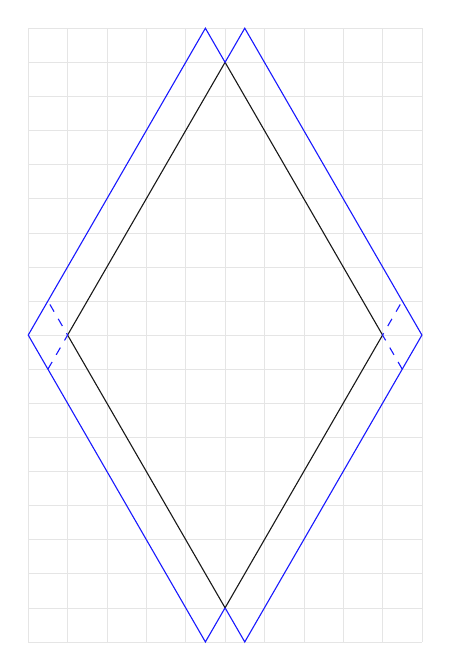
\begin{tikzpicture}[scale=0.5, yscale=.866, domain=-4:4] %%% yscale enforces sqrt(3)/2 ratio for correct triangle height
      \draw[step=1.0, color=black!10, very thin] (-5,-9) grid (5,9);
      %%% plot northern rhomb with halo-enlargement
      
      \draw[color=black!90, solid] (0,-8) -- (-4,0) -- (0,8) -- (4,0) -- (0,-8); %%% border
      \draw[color=blue!90,  solid] (0,-8) -- (-.5,-9) -- (-5,0) -- (-.5,9) -- (0,8) -- (.5,9) -- (5,0) -- (.5,-9) -- (0,-8) ; %%% border
      \draw[color=blue!90, dashed] (-4.5,-1) -- (-4,0) -- (-4.5,1) ; %%% border
      \draw[color=blue!90, dashed] (4.5,-1) -- (4,0) -- (4.5,1) ; %%% border
      
    \end{tikzpicture}
    
  \end{minipage}
  \label{fig:world_map_on_icosahedral_grid}
  \caption{Geometrical construction of the points on an icoahedron grid. Each rhomb conists of two triagles (dashed blue lines). Bisection
  of the edges leads to a hierachical sub-structure of four smaller rhombs (dashed red lines). For the reduction of data from higher
  ico-grid levels to lower ones, we need to define the Voronoi cell which is a (non-regular) hexagon (solid red line) and a (non-regular) 
  pentagon if we surround one of the twelve vertices of the icosahedron.
  The right hand side shows the implementation detail of halo-enlarged arrays. For clarity, the rhombic geometry and rotation are showm. 
  For simplicity of the implementation, the array corner cells on top and bottom are present but should never be referenced.} %%% 
\end{figure}  



  
\section{Results}\label{sec:results}
In this section we describe the results.

\section{Conclusions}\label{sec:conclusions}
We worked hard, and achieved very little.

\bibliographystyle{abbrv}
\bibliography{main}

\end{document}
